%author : berenice delcroix-oger

\documentclass[border=2pt]{standalone}
\usepackage{tikz}
\usetikzlibrary{positioning, fit, shapes, arrows, calc}

\pgfdeclarelayer{bg}    % declare background layer
\pgfsetlayers{bg,main}  % set the order of the layers (main is the standard layer)

\newcommand{\coula}{0785F2}
\newcommand{\coulb}{F29F05}
\newcommand{\coulc}{F21313}
\newcommand{\could}{E6F21F}



\definecolor{part1}{HTML}{\coula}
\definecolor{part2}{HTML}{\coulb}
\definecolor{part3}{HTML}{\coulc}
\definecolor{part4}{HTML}{\could}

\begin{document}
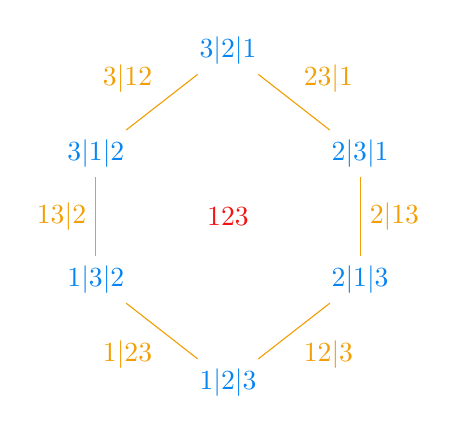
\begin{tikzpicture}
\node[part1] (123) at (0,0) {$1|2|3$};
\node[above left=1cm of 123, part1] (132) {$1|3|2$};
\node[above right=1cm of 123, part1] (213) {$2|1|3$};
\node[above=1cm of 132, part1] (312) {$3|1|2$};
\node[above=1cm of 213, part1] (231) {$2|3|1$};
\node[above right=1cm of 312, part1] (321) {$3|2|1$};
\draw[part2] (123) edge node[midway,below left, part2] {$1|23$} (132) ;
\draw[part2] (123) edge node[midway,below right, part2] {$12|3$}(213);
\draw[part2] (132) edge node[midway,left, part2](13) {$13|2$}(312);
\draw[part2] (213) edge node[midway,right, part2](2) {$2|13$}(231);
\draw[part2] (231) edge node[midway,above right, part2] {$23|1$}(321);
\draw[part2] (312) edge node[midway,above left, part2] {$3|12$}(321);
\node[part3] at ($0.5*(321)$) {$123$};
     \begin{pgfonlayer}{bg} 
\fill[part3!50] (123)--(132)--(312)--(321)--(231)--(213)--(123);
\end{pgfonlayer}
\end{tikzpicture}

\end{document}
